\documentclass[aspectratio=169,11pt]{beamer}

% Theme and colors
\usetheme{Madrid}
\usecolortheme{whale}
\setbeamertemplate{navigation symbols}{}
\setbeamertemplate{footline}[frame number]

% Packages
\usepackage[utf8]{inputenc}
\usepackage[T1]{fontenc}
\usepackage{graphicx}
\usepackage{booktabs}
\usepackage{amsmath}
\usepackage{hyperref}
\usepackage{tikz}
\usetikzlibrary{shapes,arrows,positioning,calc,fit,backgrounds}
\usepackage{siunitx}

% Bibliography
\usepackage[backend=biber,style=ieee,sorting=none]{biblatex}
\addbibresource{references.bib}

% Title information
\title[EECE5155 -- Module 3]{Local Data Processing}
\subtitle{Module 3: From Bits to Decisions at the Edge}
\author{Eduardo Baena}
\date{Spring 2026}
\institute{Northeastern University\\Department of Electrical and Computer Engineering\\
\texttt{e.baena@northeastern.edu}}

\begin{document}

% Title slide
\begin{frame}
    \titlepage
    \vspace{-1cm}
    \begin{center}
        \textbf{EECE5155: Wireless Sensor Networks and the Internet of Things}
    \end{center}
\end{frame}

% Learning Objectives
\begin{frame}{Learning Objectives}
    \textbf{By the end of this module, you should be able to:}
    
    \vspace{0.5cm}
    \begin{enumerate}
        \item \textbf{Explain} why local processing matters in IoT systems
        \item \textbf{Compare} RISC vs CISC architectures with real examples
        \item \textbf{Select} between microprocessor, microcontroller, FPGA, or ASIC
        \item \textbf{Calculate} power and performance tradeoffs from datasheets
        \item \textbf{Justify} your processing platform choice in your PES
    \end{enumerate}
    
    \vspace{0.3cm}
    \begin{block}{Engineering Question}
        Given your constraints from Module 2, which processing platform meets your requirements?
    \end{block}
\end{frame}

% Outline
\begin{frame}{Outline}
    \tableofcontents
\end{frame}

%==============================================================================
\section{Why Local Processing?}
%==============================================================================

\begin{frame}{The IoT Data Pipeline}
    \begin{center}
    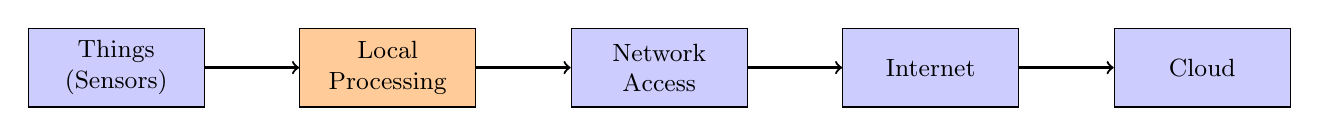
\begin{tikzpicture}[node distance=1.2cm, auto,
        block/.style={rectangle, draw, fill=blue!20, text width=2cm, text centered, minimum height=1cm, font=\small},
        highlight/.style={rectangle, draw, fill=orange!40, text width=2cm, text centered, minimum height=1cm, font=\small}]
        
        \node[block] (things) {Things\\(Sensors)};
        \node[highlight, right=of things] (proc) {Local\\Processing};
        \node[block, right=of proc] (access) {Network\\Access};
        \node[block, right=of access] (internet) {Internet};
        \node[block, right=of internet] (cloud) {Cloud};
        
        \draw[->, thick] (things) -- (proc);
        \draw[->, thick] (proc) -- (access);
        \draw[->, thick] (access) -- (internet);
        \draw[->, thick] (internet) -- (cloud);
    \end{tikzpicture}
    \end{center}
    
    \vspace{0.3cm}
    \textbf{Where does intelligence live?}
    \begin{itemize}
        \item \textbf{Cloud:} Unlimited compute, but latency + bandwidth + cost
        \item \textbf{Edge:} Limited compute, but real-time + low power + privacy
        \item \textbf{Hybrid:} Process locally, send summaries to cloud
    \end{itemize}
    
    \vspace{0.2cm}
    \textbf{Today's focus:} What happens inside the ``Thing''?
\end{frame}

\begin{frame}{Why Not Just Send Everything to the Cloud?}
    \begin{columns}[T]
        \begin{column}{0.48\textwidth}
            \textbf{The naive approach:}
            \begin{itemize}
                \item Sample sensor at 1 kHz
                \item Send all data to cloud
                \item Let cloud decide
            \end{itemize}
            
            \vspace{0.3cm}
            \textbf{The math:}
            \begin{itemize}
                \item 1 kHz $\times$ 2 bytes = 2 KB/s
                \item = 172 MB/day
                \item = 5.2 GB/month
                \item At \$0.09/GB (AWS): \$0.47/month
                \item $\times$ 1000 nodes = \$470/month
            \end{itemize}
        \end{column}
        \begin{column}{0.48\textwidth}
            \textbf{The smart approach:}
            \begin{itemize}
                \item Process locally
                \item Send only anomalies/summaries
                \item 1 packet/minute = 0.5 KB/day
            \end{itemize}
            
            \vspace{0.3cm}
            \textbf{Other benefits:}
            \begin{itemize}
                \item Latency: ms vs seconds
                \item Privacy: data stays local
                \item Reliability: works offline
                \item Power: radio is expensive
            \end{itemize}
        \end{column}
    \end{columns}
    
    \vspace{0.3cm}
    \begin{alertblock}{Engineering Decision}
        Local processing trades compute for communication. Often a good trade in IoT.
    \end{alertblock}
\end{frame}

\begin{frame}{What Can Local Processing Do?}
    \textbf{From simple to complex:}
    
    \vspace{0.3cm}
    \begin{table}
        \centering
        \small
        \begin{tabular}{@{}p{3.5cm}p{4cm}p{5cm}@{}}
            \toprule
            \textbf{Task} & \textbf{Example} & \textbf{Compute Required} \\
            \midrule
            Threshold detection & $T > 30$°C? & 1 comparison \\
            \addlinespace
            Filtering & Moving average & Few multiplies/adds \\
            \addlinespace
            Feature extraction & FFT, RMS & 100s of operations \\
            \addlinespace
            Classification & Decision tree & 10s of comparisons \\
            \addlinespace
            ML inference & TinyML model & 1000s--millions of ops \\
            \bottomrule
        \end{tabular}
    \end{table}
    
    \vspace{0.3cm}
    \textbf{Key insight:} Most IoT tasks are simple. You don't need a Raspberry Pi to check if temperature exceeds a threshold.
\end{frame}

%==============================================================================
\section{Computing Architectures}
%==============================================================================

\begin{frame}{What is a Computing Architecture?}
    \textbf{Definition:} Rules and methods describing functionality, organization, and implementation of computer systems.
    
    \vspace{0.3cm}
    \begin{columns}[T]
        \begin{column}{0.32\textwidth}
            \textbf{1. Instruction Set (ISA)}
            \begin{itemize}
                \item Machine code format
                \item Word size (8/16/32/64)
                \item Addressing modes
                \item Registers
                \item Data types
            \end{itemize}
        \end{column}
        \begin{column}{0.32\textwidth}
            \textbf{2. Microarchitecture}
            \begin{itemize}
                \item How ISA is implemented
                \item Pipeline stages
                \item Cache hierarchy
                \item Branch prediction
                \item Execution units
            \end{itemize}
        \end{column}
        \begin{column}{0.32\textwidth}
            \textbf{3. System Design}
            \begin{itemize}
                \item Memory interface
                \item Peripherals
                \item Power management
                \item Multiprocessing
                \item I/O subsystem
            \end{itemize}
        \end{column}
    \end{columns}
    
    \vspace{0.3cm}
    \begin{block}{For IoT}
        We care most about: word size, power modes, peripherals, and price.
    \end{block}
\end{frame}

\begin{frame}{CISC vs RISC: The Two Philosophies}
    \begin{columns}[T]
        \begin{column}{0.48\textwidth}
            \textbf{CISC} (Complex Instruction Set)
            \begin{itemize}
                \item Many instructions, variable length
                \item One instruction = multiple operations
                \item Memory-to-memory operations
                \item Complex addressing modes
            \end{itemize}
            
            \vspace{0.2cm}
            \textbf{Examples:}
            \begin{itemize}
                \item Intel x86 (your laptop)
                \item Intel 8051 (legacy MCU)
                \item Motorola 68000
            \end{itemize}
            
            \vspace{0.2cm}
            \textbf{IoT relevance:} Mostly legacy. 8051 still used in some cheap MCUs.
        \end{column}
        \begin{column}{0.48\textwidth}
            \textbf{RISC} (Reduced Instruction Set)
            \begin{itemize}
                \item Few instructions, fixed length
                \item One instruction = one operation
                \item Load/store architecture
                \item Simple addressing modes
            \end{itemize}
            
            \vspace{0.2cm}
            \textbf{Examples:}
            \begin{itemize}
                \item ARM Cortex-M (most IoT)
                \item RISC-V (open source, emerging)
                \item AVR (Arduino)
                \item MIPS
            \end{itemize}
            
            \vspace{0.2cm}
            \textbf{IoT relevance:} Dominant. ARM Cortex-M is everywhere.
        \end{column}
    \end{columns}
\end{frame}

\begin{frame}{Why RISC Dominates IoT}
    \begin{table}
        \centering
        \begin{tabular}{@{}lcc@{}}
            \toprule
            \textbf{Metric} & \textbf{CISC (x86)} & \textbf{RISC (ARM Cortex-M)} \\
            \midrule
            Typical power & 15--150 W & 0.1--100 mW \\
            Sleep current & N/A & 0.1--10 $\mu$A \\
            Die area & Large & Small \\
            Cost & \$50--500 & \$0.50--10 \\
            Compiler complexity & High & Low \\
            Predictable timing & Hard & Easy \\
            \bottomrule
        \end{tabular}
    \end{table}
    
    \vspace{0.3cm}
    \textbf{Key insight:} RISC's simplicity enables:
    \begin{itemize}
        \item Lower power (fewer transistors switching)
        \item Smaller die (cheaper)
        \item Predictable execution (real-time friendly)
    \end{itemize}
\end{frame}

\begin{frame}{The ARM Cortex-M Family}
    \textbf{The de facto standard for IoT microcontrollers.}
    
    \vspace{0.3cm}
    \begin{table}
        \centering
        \small
        \begin{tabular}{@{}lcccl@{}}
            \toprule
            \textbf{Core} & \textbf{Pipeline} & \textbf{MHz} & \textbf{Power} & \textbf{Use Case} \\
            \midrule
            Cortex-M0/M0+ & 2-stage & 24--48 & Ultra-low & Simple sensors \\
            Cortex-M3 & 3-stage & 72--120 & Low & General IoT \\
            Cortex-M4 & 3-stage & 80--180 & Medium & DSP, motor control \\
            Cortex-M4F & 3-stage & 80--180 & Medium & + Floating point \\
            Cortex-M7 & 6-stage & 400--600 & Higher & Edge ML, graphics \\
            Cortex-M33 & 3-stage & 100+ & Low & + Security (TrustZone) \\
            \bottomrule
        \end{tabular}
    \end{table}
    
    \vspace{0.3cm}
    \textbf{For your PES:} Most projects will use M0+ (simple) or M4 (DSP needed).
\end{frame}

%==============================================================================
\section{Specifications and Tradeoffs}
%==============================================================================

\begin{frame}{The Fundamental Tradeoffs}
    \begin{center}
    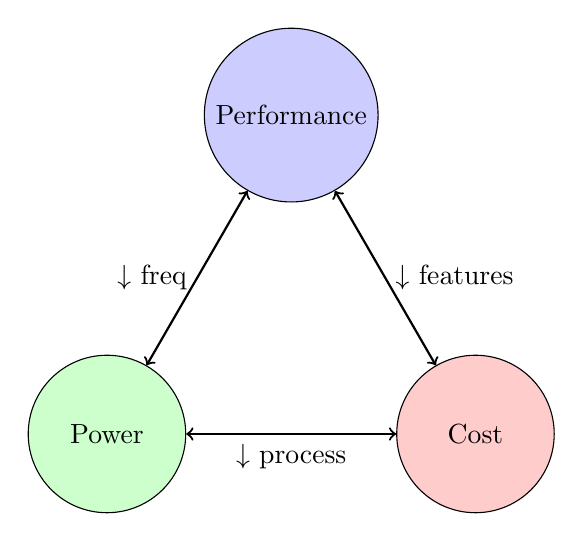
\begin{tikzpicture}[scale=0.9]
        \node[draw, circle, minimum size=2cm, fill=blue!20] (perf) at (0,3) {Performance};
        \node[draw, circle, minimum size=2cm, fill=green!20] (power) at (-2.6,-1.5) {Power};
        \node[draw, circle, minimum size=2cm, fill=red!20] (cost) at (2.6,-1.5) {Cost};
        
        \draw[<->, thick] (perf) -- (power) node[midway, left] {$\downarrow$ freq};
        \draw[<->, thick] (perf) -- (cost) node[midway, right] {$\downarrow$ features};
        \draw[<->, thick] (power) -- (cost) node[midway, below] {$\downarrow$ process};
    \end{tikzpicture}
    \end{center}
    
    \vspace{0.3cm}
    \textbf{You cannot optimize all three.} Your PES constraints determine priority:
    \begin{itemize}
        \item Battery-powered sensor? $\rightarrow$ Power first
        \item Real-time control? $\rightarrow$ Performance first
        \item 10,000 units? $\rightarrow$ Cost first
    \end{itemize}
\end{frame}

\begin{frame}{Platform Comparison: Real Numbers}
    \begin{table}
        \centering
        \footnotesize
        \begin{tabular}{@{}p{2.5cm}ccccc@{}}
            \toprule
            \textbf{Platform} & \textbf{Type} & \textbf{Price} & \textbf{Active} & \textbf{Sleep} & \textbf{Use Case} \\
            \midrule
            ATmega328P & 8-bit MCU & \$2 & 5 mA & 0.1 $\mu$A & Arduino, simple \\
            STM32L072 & Cortex-M0+ & \$3 & 3 mA & 0.3 $\mu$A & Ultra-low power \\
            STM32F4 & Cortex-M4 & \$6 & 50 mA & 2 $\mu$A & DSP, motor \\
            ESP32 & Dual-core & \$4 & 80 mA & 5 $\mu$A & WiFi/BLE \\
            nRF52840 & Cortex-M4 & \$7 & 5 mA & 0.4 $\mu$A & BLE, low power \\
            Raspberry Pi 4 & Cortex-A72 & \$35 & 3000 mA & N/A & Linux, ML \\
            \bottomrule
        \end{tabular}
    \end{table}
    
    \vspace{0.2cm}
    \textbf{Notice:}
    \begin{itemize}
        \item 1000$\times$ difference in active power (MCU vs Pi)
        \item Sleep current matters more than active for duty-cycled systems
        \item Price scales with features, not always with power
    \end{itemize}
\end{frame}

\begin{frame}{42 Years of Processor Trends}
    \textbf{Key observations from industry data:}
    
    \vspace{0.3cm}
    \begin{columns}[T]
        \begin{column}{0.48\textwidth}
            \textbf{What kept growing:}
            \begin{itemize}
                \item Transistor count (Moore's Law)
                \item Number of cores
                \item Cache sizes
            \end{itemize}
            
            \vspace{0.3cm}
            \textbf{What plateaued ($\sim$2005):}
            \begin{itemize}
                \item Clock frequency ($\sim$3--4 GHz)
                \item Single-thread performance
                \item Power per chip ($\sim$100 W)
            \end{itemize}
        \end{column}
        \begin{column}{0.48\textwidth}
            \textbf{Why frequency stopped:}
            \begin{itemize}
                \item Power $\propto$ frequency$^3$
                \item Heat dissipation limits
                \item Diminishing returns
            \end{itemize}
            
            \vspace{0.3cm}
            \textbf{IoT implication:}
            \begin{itemize}
                \item More cores don't help simple tasks
                \item Low frequency = low power
                \item MCUs benefit from process shrinks
            \end{itemize}
        \end{column}
    \end{columns}
\end{frame}

\begin{frame}{Power and Energy: The Equations}
    \textbf{Understanding the physics:}
    
    \vspace{0.3cm}
    \begin{columns}[T]
        \begin{column}{0.48\textwidth}
            \textbf{Dynamic power:}
            \[P_{dyn} = C \cdot V^2 \cdot f\]
            \begin{itemize}
                \item $C$ = capacitance (transistors)
                \item $V$ = supply voltage
                \item $f$ = frequency
            \end{itemize}
            
            \vspace{0.2cm}
            \textbf{To reduce power:}
            \begin{itemize}
                \item Lower voltage (most effective)
                \item Lower frequency
                \item Fewer transistors switching
            \end{itemize}
        \end{column}
        \begin{column}{0.48\textwidth}
            \textbf{Energy per task:}
            \[E = P \cdot t = \frac{P \cdot N_{instr}}{f}\]
            
            \vspace{0.2cm}
            \textbf{Key insight:}
            \begin{itemize}
                \item Faster $\neq$ more efficient
                \item Race-to-sleep: finish fast, sleep long
                \item Energy = power $\times$ time
            \end{itemize}
            
            \vspace{0.2cm}
            \textbf{For IoT:}
            \[E_{task} = E_{active} + E_{sleep}\]
        \end{column}
    \end{columns}
\end{frame}

\begin{frame}{Race-to-Sleep: The IoT Power Strategy}
    \textbf{Example: Read sensor, transmit, sleep}
    
    \vspace{0.3cm}
    \begin{table}
        \centering
        \small
        \begin{tabular}{@{}lccc@{}}
            \toprule
            \textbf{Strategy} & \textbf{Slow MCU} & \textbf{Fast MCU} & \textbf{Winner} \\
            \midrule
            Active current & 1 mA & 10 mA & Slow \\
            Active time & 100 ms & 10 ms & Fast \\
            Active energy & 100 $\mu$J & 100 $\mu$J & Tie \\
            Sleep current & 1 $\mu$A & 1 $\mu$A & Tie \\
            Sleep time & 59.9 s & 59.99 s & $\approx$ Tie \\
            Sleep energy & 59.9 $\mu$J & 59.99 $\mu$J & Tie \\
            \textbf{Total energy} & \textbf{160 $\mu$J} & \textbf{160 $\mu$J} & \textbf{Tie} \\
            \bottomrule
        \end{tabular}
    \end{table}
    
    \vspace{0.3cm}
    \textbf{Conclusion:} For duty-cycled IoT, sleep current dominates. Active power matters less than you think.
\end{frame}

%==============================================================================
\section{Microprocessor vs Microcontroller}
%==============================================================================

\begin{frame}{The Fundamental Difference}
    \begin{columns}[T]
        \begin{column}{0.48\textwidth}
            \textbf{Microprocessor (MPU)}
            \begin{center}
            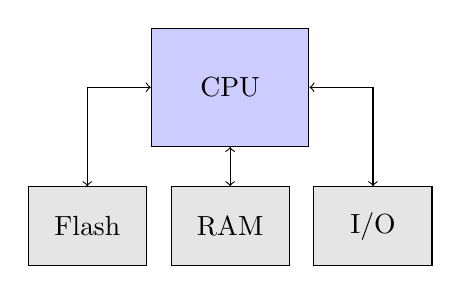
\begin{tikzpicture}[scale=0.7]
                \node[draw, rectangle, minimum width=2cm, minimum height=1.5cm, fill=blue!20] (cpu) {CPU};
                \node[draw, rectangle, minimum width=1.5cm, minimum height=1cm, fill=gray!20, below=0.5cm of cpu] (ram) {RAM};
                \node[draw, rectangle, minimum width=1.5cm, minimum height=1cm, fill=gray!20, left=0.3cm of ram] (flash) {Flash};
                \node[draw, rectangle, minimum width=1.5cm, minimum height=1cm, fill=gray!20, right=0.3cm of ram] (io) {I/O};
                \draw[<->] (cpu) -- (ram);
                \draw[<->] (cpu) -| (flash);
                \draw[<->] (cpu) -| (io);
            \end{tikzpicture}
            \end{center}
            \begin{itemize}
                \item CPU only on chip
                \item External memory, I/O
                \item Flexible, general purpose
                \item Higher power, cost
                \item Examples: RPi, BeagleBone
            \end{itemize}
        \end{column}
        \begin{column}{0.48\textwidth}
            \textbf{Microcontroller (MCU)}
            \begin{center}
            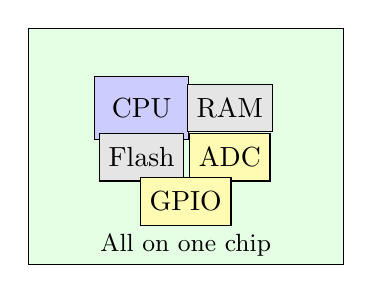
\begin{tikzpicture}[scale=0.7]
                \node[draw, rectangle, minimum width=4cm, minimum height=3cm, fill=green!10] (mcu) {};
                \node[draw, rectangle, minimum width=1.2cm, minimum height=0.8cm, fill=blue!20] at (-0.8,0.7) {CPU};
                \node[draw, rectangle, minimum width=1cm, minimum height=0.6cm, fill=gray!20] at (0.8,0.7) {RAM};
                \node[draw, rectangle, minimum width=1cm, minimum height=0.6cm, fill=gray!20] at (-0.8,-0.2) {Flash};
                \node[draw, rectangle, minimum width=1cm, minimum height=0.6cm, fill=yellow!30] at (0.8,-0.2) {ADC};
                \node[draw, rectangle, minimum width=1cm, minimum height=0.6cm, fill=yellow!30] at (0,-1) {GPIO};
                \node at (0,-1.8) {\small All on one chip};
            \end{tikzpicture}
            \end{center}
            \begin{itemize}
                \item CPU + RAM + Flash + I/O
                \item Integrated peripherals
                \item Compact, low power
                \item Examples: STM32, ESP32
            \end{itemize}
        \end{column}
    \end{columns}
\end{frame}

\begin{frame}{When to Use Which?}
    \begin{table}
        \centering
        \begin{tabular}{@{}p{4cm}cc@{}}
            \toprule
            \textbf{Requirement} & \textbf{MCU} & \textbf{MPU} \\
            \midrule
            Battery powered & \checkmark & \\
            Real-time control & \checkmark & \\
            Simple sensing & \checkmark & \\
            Cost $<$\$10 & \checkmark & \\
            \addlinespace
            Run Linux & & \checkmark \\
            Complex ML & & \checkmark \\
            GUI/Display & & \checkmark \\
            Network stack & & \checkmark \\
            \addlinespace
            WiFi + simple logic & \multicolumn{2}{c}{ESP32 (hybrid)} \\
            \bottomrule
        \end{tabular}
    \end{table}
    
    \vspace{0.3cm}
    \begin{alertblock}{Common Mistake}
        Using Raspberry Pi for a task that needs 3 GPIO reads and 1 UART write. That's a \$2 MCU job.
    \end{alertblock}
\end{frame}

\begin{frame}{CPU vs GPU vs DSP}
    \begin{columns}[T]
        \begin{column}{0.32\textwidth}
            \textbf{CPU}
            \begin{itemize}
                \item Few cores (1--8)
                \item General purpose
                \item Sequential tasks
                \item Branching, control
            \end{itemize}
            
            \vspace{0.2cm}
            \textbf{IoT use:}
            \begin{itemize}
                \item Control logic
                \item State machines
                \item Protocol handling
            \end{itemize}
        \end{column}
        \begin{column}{0.32\textwidth}
            \textbf{GPU}
            \begin{itemize}
                \item Many cores (100s--1000s)
                \item Parallel SIMD
                \item Graphics, ML
                \item High power
            \end{itemize}
            
            \vspace{0.2cm}
            \textbf{IoT use:}
            \begin{itemize}
                \item Edge ML (Jetson)
                \item Video processing
                \item Rarely needed
            \end{itemize}
        \end{column}
        \begin{column}{0.32\textwidth}
            \textbf{DSP}
            \begin{itemize}
                \item Optimized for signals
                \item MAC instructions
                \item Fixed-point math
                \item Low power
            \end{itemize}
            
            \vspace{0.2cm}
            \textbf{IoT use:}
            \begin{itemize}
                \item Audio processing
                \item Filtering
                \item Cortex-M4 has DSP
            \end{itemize}
        \end{column}
    \end{columns}
\end{frame}

\begin{frame}{ASIC vs FPGA}
    \begin{columns}[T]
        \begin{column}{0.48\textwidth}
            \textbf{ASIC} (Application-Specific IC)
            \begin{itemize}
                \item Custom silicon for one task
                \item Lowest power, smallest size
                \item Highest performance
                \item \$100k--\$1M+ NRE cost
                \item No flexibility after fab
            \end{itemize}
            
            \vspace{0.2cm}
            \textbf{When to use:}
            \begin{itemize}
                \item Millions of units
                \item Extreme power/perf needs
                \item Example: Bitcoin miners
            \end{itemize}
        \end{column}
        \begin{column}{0.48\textwidth}
            \textbf{FPGA} (Field-Programmable)
            \begin{itemize}
                \item Reconfigurable logic
                \item Moderate power, larger
                \item Good performance
                \item \$10--\$1000 per chip
                \item Can change after deployment
            \end{itemize}
            
            \vspace{0.2cm}
            \textbf{When to use:}
            \begin{itemize}
                \item Prototyping ASICs
                \item Custom interfaces
                \item Parallel processing
                \item Example: SDR, crypto
            \end{itemize}
        \end{column}
    \end{columns}
    
    \vspace{0.3cm}
    \textbf{For most IoT projects:} MCU is sufficient. FPGA/ASIC are overkill.
\end{frame}

%==============================================================================
\section{Non-Conventional Computing}
%==============================================================================

\begin{frame}{Beyond Von Neumann}
    \textbf{Emerging paradigms (for awareness, not your PES):}
    
    \vspace{0.3cm}
    \begin{columns}[T]
        \begin{column}{0.32\textwidth}
            \textbf{Neuromorphic}
            \begin{itemize}
                \item Brain-inspired
                \item Analog signals
                \item Event-driven
                \item Ultra-low power
                \item Intel Loihi, IBM TrueNorth
            \end{itemize}
            
            \vspace{0.2cm}
            \textbf{IoT potential:}\\
            Always-on sensing
        \end{column}
        \begin{column}{0.32\textwidth}
            \textbf{Quantum}
            \begin{itemize}
                \item Qubits (superposition)
                \item Entanglement
                \item Specific algorithms
                \item Cryogenic cooling
                \item IBM, Google, IonQ
            \end{itemize}
            
            \vspace{0.2cm}
            \textbf{IoT potential:}\\
            Crypto (QKD)
        \end{column}
        \begin{column}{0.32\textwidth}
            \textbf{Molecular/DNA}
            \begin{itemize}
                \item Biological computing
                \item Massive parallelism
                \item Very slow
                \item Research stage
            \end{itemize}
            
            \vspace{0.2cm}
            \textbf{IoT potential:}\\
            Biosensors
        \end{column}
    \end{columns}
    
    \vspace{0.3cm}
    \textbf{Reality check:} For your projects, stick with ARM Cortex-M.
\end{frame}

%==============================================================================
\section{Selecting Your Platform}
%==============================================================================

\begin{frame}{Decision Framework for Your PES}
    \textbf{Step-by-step selection:}
    
    \vspace{0.3cm}
    \begin{enumerate}
        \item \textbf{List your constraints} (from Module 2)
        \begin{itemize}
            \item Power budget, cost target, required peripherals
        \end{itemize}
        
        \item \textbf{Determine processing needs}
        \begin{itemize}
            \item Simple threshold? $\rightarrow$ Any MCU
            \item DSP/filtering? $\rightarrow$ Cortex-M4
            \item ML inference? $\rightarrow$ Cortex-M4/M7 or MPU
        \end{itemize}
        
        \item \textbf{Check peripheral requirements}
        \begin{itemize}
            \item ADC channels, resolution, speed
            \item Communication: SPI, I2C, UART, USB
            \item Timers, PWM, DMA
        \end{itemize}
        
        \item \textbf{Verify power budget}
        \begin{itemize}
            \item Calculate from datasheet (like Module 2)
        \end{itemize}
        
        \item \textbf{Document your choice with justification}
    \end{enumerate}
\end{frame}

\begin{frame}{Example: MCU Selection for Temperature Monitor}
    \textbf{Requirements:}
    \begin{itemize}
        \item 2-year battery life (47 $\mu$A budget)
        \item 1 temperature sensor (1-Wire)
        \item LoRa radio (SPI)
        \item Cost $<$\$5
    \end{itemize}
    
    \vspace{0.3cm}
    \begin{table}
        \centering
        \small
        \begin{tabular}{@{}lcccl@{}}
            \toprule
            \textbf{MCU} & \textbf{Sleep} & \textbf{Active} & \textbf{Cost} & \textbf{Verdict} \\
            \midrule
            ATmega328P & 0.1 $\mu$A & 5 mA & \$2 & OK, but 8-bit \\
            STM32L072 & 0.3 $\mu$A & 3 mA & \$3 & \textbf{Best fit} \\
            ESP32 & 5 $\mu$A & 80 mA & \$4 & Overkill, power \\
            nRF52832 & 0.3 $\mu$A & 5 mA & \$5 & Good, but BLE focus \\
            \bottomrule
        \end{tabular}
    \end{table}
    
    \vspace{0.2cm}
    \textbf{Selection:} STM32L072 -- lowest active power, good sleep, SPI for LoRa, \$3.
\end{frame}

\begin{frame}{What Your PES Must Include}
    \textbf{Section 6: Processing Platform}
    
    \vspace{0.3cm}
    \begin{enumerate}
        \item \textbf{Platform selected:} Specific part number (e.g., STM32L072CZT6)
        
        \item \textbf{Justification:}
        \begin{itemize}
            \item Why this architecture? (Cortex-M0+ for low power)
            \item Why this specific part? (peripherals, package, availability)
        \end{itemize}
        
        \item \textbf{Power analysis:} (from datasheet)
        \begin{itemize}
            \item Sleep current: X $\mu$A (DS page Y)
            \item Active current: X mA @ Y MHz (DS page Z)
            \item Calculated average: X $\mu$A
        \end{itemize}
        
        \item \textbf{Peripheral mapping:}
        \begin{itemize}
            \item SPI1 $\rightarrow$ LoRa radio
            \item GPIO PA5 $\rightarrow$ 1-Wire sensor
            \item USART2 $\rightarrow$ Debug console
        \end{itemize}
    \end{enumerate}
\end{frame}

%==============================================================================
\section{Summary}
%==============================================================================

\begin{frame}{Module Summary}
    \textbf{Key Takeaways:}
    
    \vspace{0.3cm}
    \begin{enumerate}
        \item \textbf{Local processing} reduces bandwidth, latency, power, and cost
        \item \textbf{RISC (ARM Cortex-M)} dominates IoT for good reasons
        \item \textbf{MCU vs MPU:} Use MCU unless you need Linux or heavy ML
        \item \textbf{Power tradeoffs:} Sleep current often matters more than active
        \item \textbf{Selection process:} Constraints $\rightarrow$ requirements $\rightarrow$ datasheet $\rightarrow$ choice
    \end{enumerate}
    
    \vspace{0.3cm}
    \begin{block}{For Your PES}
        Document your MCU selection with:
        \begin{itemize}
            \item Part number and datasheet reference
            \item Power budget calculation
            \item Peripheral mapping
            \item Justification tied to your constraints
        \end{itemize}
    \end{block}
\end{frame}

\begin{frame}{What's Next}
    \begin{columns}[T]
        \begin{column}{0.48\textwidth}
            \textbf{Module 4: Data Communication}
            \begin{itemize}
                \item Wireless protocols
                \item LoRa, BLE, Zigbee, WiFi
                \item Protocol selection criteria
                \item Link budgets
                \item Network topologies
            \end{itemize}
        \end{column}
        \begin{column}{0.48\textwidth}
            \textbf{Your Task:}
            \begin{itemize}
                \item Select MCU for your project
                \item Calculate power budget
                \item Map peripherals
                \item Update PES Section 6
            \end{itemize}
        \end{column}
    \end{columns}
    
    \vspace{0.5cm}
    \begin{center}
        \Large
        \textbf{Questions?}
    \end{center}
\end{frame}

%==============================================================================
% References
%==============================================================================

\begin{frame}[allowframebreaks]{References}
    \printbibliography
\end{frame}

\end{document}
